\documentclass[a4paper]{article}

%% Language and font encodings
%\usepackage[english]{babel}
%\usepackage[utf8x]{inputenc}
%usepackage[T1]{fontenc}

%% Sets page size and margins
\usepackage[a4paper,top=3cm,bottom=2cm,left=3cm,right=3cm,marginparwidth=1.75cm]{geometry}

%% Useful packages
\usepackage{amsmath}
\usepackage{graphicx}
\usepackage[colorinlistoftodos]{todonotes}
\usepackage[colorlinks=true, allcolors=blue]{hyperref}
\usepackage{bmpsize}

\newtheorem{define}{Definition}
\newtheorem{thm}{Theorem}
\newtheorem{property}{Property}
\newtheorem{lemma}{Lemma}
\newtheorem{cor}{Corollary}

\newcommand{\cks}[1]{\textcolor{red}{cks: #1}}
\newcommand{\ab}[1]{\textcolor{cyan}{ab: #1}}

\title{A Recursive Strategy for Symbolic Execution Expressed in Coq}
\author{A. Byrnes and C. Sturton}

\begin{document}
\maketitle

\begin{abstract}
Prior work has proposed the use of symbolic execution for the security
validation of a processor design. The approach uses a recursive search strategy
that is designed to counter the exponential path growth inherent in multi-cycle
processor execution. In this work, we examine the search strategy in order to prove its correctness. We formulate the
strategy in Coq, and we find that the
strategy as proposed is not guaranteed to produce correct results---that is, the
search may find a symbolic path for which no concrete path from the processor's initial state
to the given error state exists. We tighten one of the requirements of the
search strategy and make explicit an unstated assumption of the strategy. We then prove the modified strategy correct. 
\end{abstract}

\section{Introduction}
\cks{15 pages, excl. bib, excl. appdx}
Researchers have recently begun exploring the use of software-style symbolic execution for the
verification of hardware designs~\cite{paperswecite}. Symbolic execution has a proven track record in the software community as a
bug-finding tool~\cite{} and as an aid in formal verification~\cite{}. However,
handling the complexity and search space of hardware designs has been a
challenge. In response to this challenge a recent paper proposed a recursive
search strategy~\cite{fms}. The strategy has been demonstrated to be
practical~\cite{coppelia}, but the soundness of the approach has never been
demonstrated. A proof of correctness is needed.


In this paper we prove the validity of the recursive search strategy for the
symbolic execution of hardware designs. We formalize a model of symbolic
execution and prove that a recursive search strategy is sound: A list of
constraints returned by a successful search defines a set of concrete input
sequences, each of which will take the processor from its initial reset state to
an error state.

Our goal is to validate the search strategy itself rather than any one implementation
of it. Therefore we decouple our model of symbolic execution from a particular
coding language to be symbolically executed. The structure of the model is built
around the three fundamental properties of symbolic execution as first laid out
by King in 1976~\cite{}.

Our insight is that by building a model of symbolic execution based purely on
the three fund...~\cite{}, we can decouple the proof of the validity of the
search strategy from a proof about the correctness of any one particular
symbolic execution engine. Any symbolic exploration that uses the search
strategy we study here will produce sound results \cks{this is too strong}.
We find that the search strategy as originally proposed is not sound---that is, the
search may find a symbolic path for which no concrete path from the processor's initial state
to the given error state exists. We tighten the requirements of two of the three
requirements of the strategy and then prove the modified strategy correct.

We take advantage of the fact that/
Our insight is that both the recursive search strategy and symbolic execution
have clearly defined properties that are sufficient or assumed sufficient to
make the approach work.  make the a proof of soundness of the search strategy depends on a 

We use XXX, Coq's modeling language to build an abstract model of symbolic execution that 



\section{Prior Work}
Symbolic execution was first formally defined by King in 1976~\cite{king1976symbolic} and has
been widely adopted by the software engineering and software security
communities. (See Schwartz et al.~\cite{schwartz2010all} for a recent survey.)

Symbolic execution has since shown practical value through implementations. Anand et al. introduced a tool JPF-SE that works as an extension of the Java PathFinder model checker to allow for symbolic execution of Java programs~\cite{anand2007jpf}.  P{\u{a}}s{\u{a}}reanu et al. later introduced the tool Symbolic PathFinder that also utilizes Java Path Finder to symbolically execute Java bytecode~\cite{puasuareanu2010symbolic}. Noller et al. recently released a tool that utilizes Java PathFinder to perform ``shadow symbolic execution'' on Java bytecode~\cite{Noller2018}.

\subsection{Use of Symbolic Execution in Hardware}
In addition to the paper by Zhang and Sturton that lays out the three-part
strategy we prove here~\cite{zhang2018recursive}, there are a handful of papers that examine
the use of symbolic execution in hardware. In a subsequent paper, Zhang et
al.~\cite{zhang2018recursive} make use of their recursive strategy to find new security
vulnerabilities in processor designs. Their work demonstrates that the strategy
is useful in practice.

Prior work first explored the use of software-style symbolic execution for hardware designs. The STAR tool combines symbolic and concrete simulation of hardware designs to
provide high statement and branch coverage~\cite{liu2009star}; PATH-SYMEX uses
forward symbolic execution applied to an ANSI-C model of the hardware
design~\cite{mukherjee2015hardware}. Both tools use a forward search strategy
and have limits on how deep or broadly they can search.

\subsection{Formalization of Symbolic Execution}
Arusoaie et al. \cks{summarize gist of this work and point out differences from
  our work.} \cite{arusoaie2014generic}, \cite{arusoaie2015symbolic}. Lucanu et
al. \cks{did something closely related to the first two papers.} \cite{lucanu2017generic}

\subsection{Backward Search Strategies in Symbolic Execution}

A backward search strategy for symbolic execution of software has been
studied~\cite{ma2011directed,chandra09,dinges04,charreteur10}. There the approach is to search
backward through function call chains from a goal line of code to the program's
entry point. The strategy is hindered by complications that arise in software,
such as floating point calculations and external method calls. To the best of our knowledge, the strategy has not been formalized
in the software community, nor its validity proven. \cks{double check these citations.}


\section{Background}
\cks{SE w/formalization; statement of King properties; SE for HW; explanation of
  RecSE; statement of 3 RecSE properties}
\subsection{Symbolic Execution}
In symbolic execution the final parameters to a program's entry point are
assigned symbolic values. The symbolic execution engine simulates each line of
code, using the symbolic values in place of the usual concrete literals. As
execution continues the resulting symbolic expressions propagate throughout the program's
state. The symbolic execution engine
maintains the current, partially symbolic state of the program and the current
\emph{path condition}. The path condition is a conjunction of propositions over
input and state variables that define the path through the program code taken to
reach the current state. Figure~\ref{fig:se} demonstrates the idea. 

For example, for the code in
Figure~\ref{fig:sea}, if $\mathtt{reset}$ and $\mathtt{count}$ are initialized
with the symbolic values $r_0$ and $c_0$, respectively, then after symbolically
executing lines 1, 3, and 4 count may be set to the symbolic expression $c_0 +
1$ as shown in Figure~\ref{fig:sec}. In addition to the (partially) symbolic
state that is maintained, a symbolic execution engine keeps track of the
\emph{path condition}. The path condition is a conjunction of propositions that
accrue at each conditional branch point in the program. There is one path
condition per path of execution through the code. In Figure~\ref{fig:sec} the
path condition for the path through lines 1, 3, 4, 5, 6 is shown. When execution
reaches the $\mathtt{ERROR}$ at line 6 the path condition is $\mathit{pc} := r_0
== 0 \wedge c_0 + 1 > 3$. This expression can then be solved using a standard,
off-the-shelf SMT solver to find a satisfying solution, say $r_0 := 0$ and $c_0
:= 3$. Substituting these values for $\mathtt{reset}$ and $\mathtt{count}$,
respectively and executing the code concretely could cause execution to follow
the same path as was followed symbolically.

\cks{Brain dump a bunch of mostly terrible text to get started.}
We model the processor as a vector $R$ of state registers $R = <r_0, r_1,
\ldots, r_n>$. At each step of execution (clock cycle) the valuation of each
register may change. New state is determined by the Boolean and bitvector
arithmetic combination of current state plus input values. $\forall m, r'_m =
\delta(R,I)$.

In concrete execution registers hold concrete values $(v_0, v_1, \ldots, v_n)$
at each clock cycle. In symbolic execution the concrete values are replaced with
symbolic values $(\phi_0, \phi_1, \ldots, \phi_n)$ and so are input values.
As execution continues, symbolic values propagate through the design.

The symbolic state is modeled as a tuple $\psi := (S,\pi)$ where $S$ is the
vector of registers containing a combination of symbolic and concrete state $S
:= <s_0, s_1, \ldots, s_n>$. As execution continues, symbolic values propagate
through the design.

When execution begins the path constraint is initialized to $\mathtt{\textsc{true}}$. At
each conditional branch the condition $c$ is evaluated. If $\pi \rightarrow c$
the $\mathtt{then}$ branch is taken and the path constraint is
updated $\pi := \pi \wedge c$. If $\pi \rightarrow \not c$ the $\mathtt{else}$
branch is taken and the path constraint is updated $\pi := \pi \wedge \not
c$. If neither $\pi \rightarrow c$ nor $\pi \rightarrow \not c$ hold, then both
branches are possible. Execution forks and both branches are explored in turn
with the path condition updated appropriately for each branch.
\cks{Need to introduce trees}

King formalized the use of symbolic execution~\cite{??} and describes three
properties provided by symbolic execution. We name and summarize the properties
here.
\begin{property}[Sound Paths]
  \label{prop:kingsound}
  The path constraint $\pi$ never becomes unsatisfiable. This means that at each
  leaf node the path constraint $\pi$ assoicated with that leaf node has at
  least one concrete valuation which would drive execution down the same path of
  execution.
\end{property}
\begin{property}[Unique Paths]
  \label{prop:kingunique}
The path constraints $\pi_1$ and $\pi_2$ associated with any two paths of the
tree are mutually unsatisfiable. In other words, there exists no concrete
valuation that could drive execution down two distinct paths of the symbolic
execution tree.
\end{property}
\begin{property}[Commutativity]
  \cks{Todo}
\end{property}

\subsection{Symbolic Execution of Hardware Designs}






\section{System Framework}
\section{Verification Approach}
%figures : 
We give a basic outline of our proof of our correctness theorem.

We want to show that $\mathtt{execute\_tree\_list} (tree\_list) \in error\_states$.

We prove this by first proving Theorem \ref{thm:etl}.

\begin{proof}[Theorem \ref{thm:etl}]
This is a proof by induction on the size of $tree\_list$.

For our base case we show that if $tree\_list$ is of length $1$, then $\mathtt{execute\_tree\_list} (tree\_list) \in \mathtt{concretize\_leaf} (\mathtt{last\_element} (tree\_list))$.


To prove this we use the following set property (which we verify in Coq):

\begin{theorem}
$\forall$ inputs $i$,
If $A \in B$ and 
$\forall x \in B$, \concexecution($x, i$) $\in C$, then  \concexecution($A, i$) $\in$ $C$.
\label{thm:set2}
\end{theorem}

If $tree\_list$ is of length $1$, we know we are executing from the initial concrete state of the system. Therefore, we consider the following properties:
\begin{itemize}
\item $init\_conc\_state \in 
  \mathtt{concretize\_root} (\mathtt{last\_element} (tree\_list))$. (Property $1$)
 \item $ \forall$ inputs $i$, 
 $\forall x \in
  \mathtt{concretize\_root} (\mathtt{last\_element} (tree\_list))$,  \\
 $ \concexecution(x, i) \in \mathtt{concretize\_leaf}(\mathtt{last\_element}(tree\_list))$.
\end{itemize}

Now, using Theorem \ref{thm:set2}, we conclude that $\concexecution(init\_conc\_state) \in \mathtt{concretize\_leaf}(\mathtt{last\_element}(tree\_list))$.

Our inductive hypothesis is  $\mathtt{execute\_tree\_list} (tree\_list') \in \mathtt{concretize\_leaf} (\mathtt{last\_element}(tree\_list'))$ where $tree\_list'$ is $tree\_list$ with the last element removed.

We want to show that if our inductive hypothesis holds, then $\mathtt{execute\_tree\_list} (tree\_list) \in \mathtt{concretize\_leaf}(tree\_list)$.

In order to prove this, we must prove the following lemma:
\begin{lemma} 
\label{lem:etl}
$\mathtt{execute\_tree\_list} (tree\_list') \in \mathtt{concretize\_root} (\mathtt{last\_element} (tree\_list))$.
\end{lemma}
\begin{proof}[Lemma \ref{lem:etl}]
We prove this using the following set property (which we verify in Coq):

\begin{theorem} \label{thm:set1}
If $A \in B$ and $B \subseteq C$, then $A \in C$.
\end{theorem}

We know:
\begin{itemize}
\item$ \mathtt{execute\_tree\_list}(tree\_list') \in
        \mathtt{concretize\_leaf} (\mathtt{last\_element}(tree\_list')) $. (Inductive Hypothesis)
\item 
$\mathtt{concretize\_leaf} (\mathtt{last\_element}(tree\_list')) \subseteq \mathtt{concretize\_root} (\mathtt{last\_element} (tree\_list))$. (Property $3$)
 \end{itemize}
 
 So, using Theorem \ref{thm:set1}, we conclude that $\mathtt{execute\_tree\_list} (tree\_list') \\ 
 \in 
 \mathtt{concretize\_root} (\mathtt{last\_element} (tree\_list))$. \qed
\end{proof}

Now, to prove our inductive step, we know:
\begin{itemize}
\item $\mathtt{execute\_tree\_list} (tree\_list') \in \mathtt{concretize\_leaf} (\mathtt{last\_element}(tree\_list'))$. (Lemma \ref{lem:etl})
\item if $x \in \mathtt{concretize\_root}(\mathtt{last\_element}(tree\_list))$, then \\
  $\concexecution(x, get\_input (l.\pathcondition)) \in \mathtt{concretize\_leaf}(\mathtt{last\_element}(tree\_list))$,
where $l$ is a leaf of $\mathtt{last\_element}(tree\_list)$. (Lemma \ref{cop})
\item $\mathtt{concretize\_leaf}(t) \neq \{\} $. (Property $3'$)
\end{itemize}

So, using Theorem \ref{thm:set2}, we can conclude that \\
$\mathtt{execute\_tree\_list} (tree\_list) \in \mathtt{concretize\_leaf} (\mathtt{last\_element}(tree\_list))$. \qed
\end{proof}

Now, we prove our correctness property.

\begin{proof}[Theorem \ref{thm:sufficiency}]
We know:
\begin{itemize}
\item $\mathtt{execute\_tree\_list}(tree\_list) \in \mathtt{concretize\_leaf}(\mathtt{last\_element}(tree\_list))$. (Theorem \ref{thm:etl})
\item $\mathtt{concretize\_leaf} (\mathtt{last\_element} (tree\_list)) \subseteq error\_states$. (Property $2'$)
\end{itemize}
so, using Theorem \ref{thm:set1}, we conclude
$\mathtt{execute\_tree\_list} (tree\_list) \in error\_states$. \qed
\end{proof}

The reason we need Property $2'$ is because Property $2$ is not sufficient. 
This is because if $\mathtt{execute\_tree\_list} (tree\_list) \in \mathtt{concretize\_leaf} (\mathtt{last\_element}(tree\_list))$ and \\
$\mathtt{concretize\_leaf} (\mathtt{last\_element} (tree\_list)) \cap error\_states \neq \{\}$, we could get the case where
$\mathtt{execute\_tree\_list} (tree\_list) \notin error\_states$, as shown in Figure \ref{fig:Prop2}.

\begin{figure}
  \centering
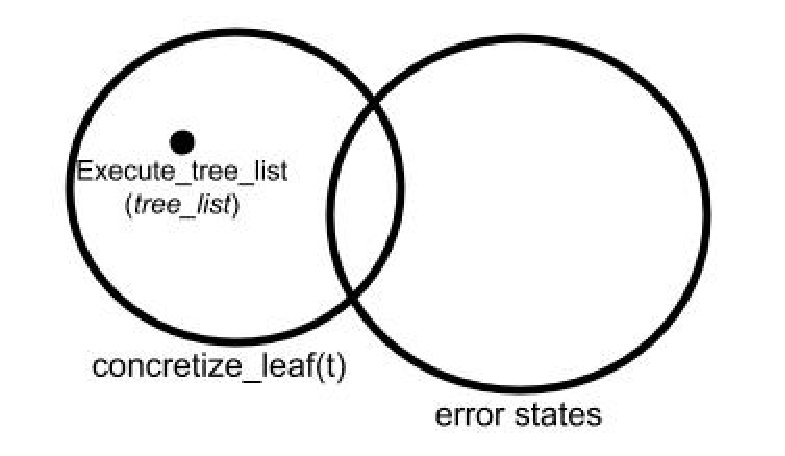
\includegraphics[width=.4\textwidth]{prop2.eps}
\caption{Example of Property $2$ not being sufficient to show $\mathtt{execute\_tree\_list} (tree\_list) \in error\_states$.}
\label{fig:Prop2}
\end{figure}





\section{Conclusion}

\input scraptext
%% \input introduction
%% \input background
%% \input proofdesign
%% \input relatedwork
%% \input conclusion


\bibliographystyle{alpha}
\bibliography{references}

\end{document}
